\chapter{Cadre général du projet}
\section*{Introduction}
Dans ce chapitre, nous allons présenter le cadre général du projet. Tout d'abord, nous présentons l'organisme d'accueil "Dqlick". Puis nous passons à la description du contexte de notre travail. Ensuite, nous expliquons la méthodologie du travail que nous avons adopté.

% Une section

% Exemple d'une section qui porte une référence à une bibliographie
% NB: il faut bien suivre le syntaxe pour ne pas tomber dans le cas où il y a une référence dans la table des matières.
\section {Présentation de l’organisme d’accueil Dqlick}

Dqlick est un éditeur de logiciels en marque blanche, permettant de couvrir tout le périmètre des activités des assurances, de gérer l’ensemble des contrats, d’innover en terme de gamme de produits tout en réduisant les contraintes de délais et de coûts. Dqlick s'adapte à tous les métiers avec un catalogue riche en fonctionnalités.
 


\item Dqlick met à la disposition de sa clientèle différents services :

\begin{itemize}[font=\normalsize]

\item Digitales  services 

\item User experience Design 

\item GED & Dématérialisation 

\item DATA ANALYTICS

\item AMOA & QA

\end{itemize}

\item Dqlick fournit des solutions dans le domaine Assurtech.

\begin{itemize}[font=\normalsize]
\item\textbf{ Des solutions innovatives:} Créativité et inspiration à travers la recherche et l'analyse des tendances.

\item \textbf{Des solutions productives:} Solution robuste, fiable et évolutive permettant de piloter efficacement les activités.

\item \textbf{Des solutions customisées:} Solution adéquate pour toute organisation et pour chaque besoin.

\item \textbf{Des solutions dediées pour les utilisateurs:}  web
user-Friendly
\end{itemize}

\section{Pr\'esentation du projet }
\subsection{Context du projet}
Notre stage a été réalisé dans le cadre d'un stage ingénieur en vue d'apprendre et  d’obtenir  le diplôme d’ingénieur en informatique à l’école nationale d’ingénieurs de Carthage.\\
Le travail qu'on nous a confié est la gestion des agences dans le cadre d'une application AssurTech.




\subsection{Solution et objectifs }
Dqlick propose un système de gestion de contrats santé et prévoyance unique pour les
organismes d'assurance santé qui s'adapte en fonction de leurs besoins. Grace à ses équipes dédiées et motivées, Dqlick offre une qualité de services optimale à vos assurés.

\item Les principales fonctionnalités que notre application doit assurer :
\begin{itemize}[font=\normalsize]
\item\textbf {Une architecture web élégante et dynamique}
\item\textbf{Productivité: } Plus de qualité, de productivité et de réactivité, au meilleur coût
\item\textbf{Suivi des activités :}  Des outils de reporting mis à disposition des assureurs afin d’effectuer un pilotage chiffré et personnalisé.
\item\textbf{Service Fiable & Complet :} Couvre toute la chaîne de valeur (assureurs, Partenaires, Distributeurs, Gestionnaires...)
\end{itemize}

\section{M\'ethodologie}
L’adoption d’une méthode de gestion d’un projet est une étape primordiale pour les membres d’une équipe afin d’atteindre conjointement les objectifs attendus dans les délais prévus.
L’équipe adopte déjà l’approche Scrum, particulièrement la méthode Scrum, nous avons donc suivi cette méthode pour la gestion de notre projet.

\subsection{Approche agile}
La méthodologie agile est une approche itérative et incrémentale qui offre une grande capacité d’adaptation aux changements et aux imprévus. Le but principal d’Agile est de livrer une version fonctionnelle du produit entre les mains du client aussi vite que possible.

\begin{itemize}[label=\textbullet,font=\normalsize]
\addtolength{\itemindent}{1cm}
\item \textbf{Principes Agile :}
Le manifeste agile concrétise 12 principes importants : 
\begin{figure}[H]
\centering
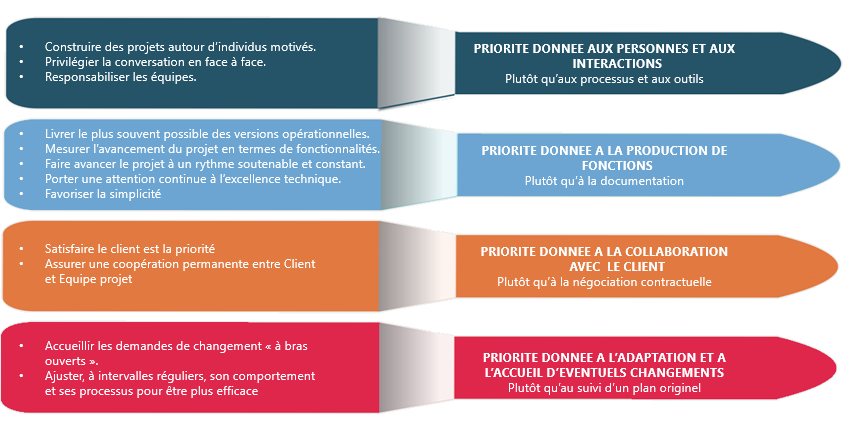
\includegraphics[width=1\columnwidth]{images/principes_agile.png}
\caption{les principes Agile}
\label{fig:les principes Agile}
\end{figure} 

\item \textbf{Processus de développement :}
Agile suit un développement de versions succes- \\ sives appelées incréments qui ajoutent et changent des fonctionnalités nécessaires au fil du temps pour fournir un produit plus robuste. Chaque module successif est planifié, codé, testé et complété sur de courtes sessions de deux à quatre semaines comme le montre la figure ci-dessous.
\begin{figure}[H]
\centering
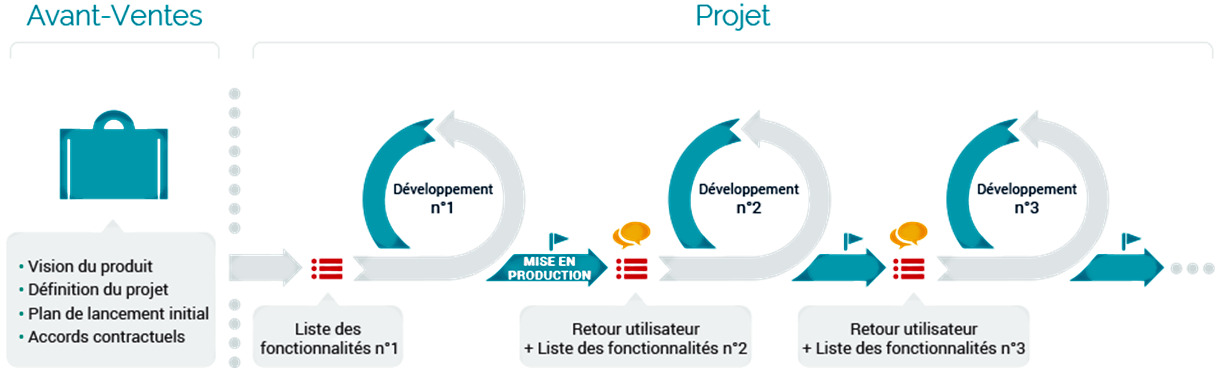
\includegraphics[width=1\columnwidth]{images/processus_agile.png}
\caption{cycle de vie Agile}
\label{fig:Mod-Enseig}
\end{figure} 
\end{itemize}

\subsection{SCRUM}
La méthode Scrum est la méthode agile la plus utilisée, éprouvée et documentée. Elle est considérée comme un cadre simple pour la gestion des projets complexes qui se base sur la transparence, l’adaptation et l’inspection. Elle s’appuie sur le découpage du projet en itérations, nommés sprints. Ce dernier représente des « user stories » à réalisées dans une durée fixe de 1 à 4 semaines.
Dans notre équipe scrum nous avons cinq rôles : 
\begin{itemize}[label=\textbullet,font=\normalsize]
\addtolength{\itemindent}{1cm}
\item \textbf{Le product owner : } le représentant officiel du client, il définit les besoins du produit et rédige les spécifications
\item \textbf{Le scrum master :} Chargé de veiller à la mise en application de la méthode et au respect de ses objectifs.
\item \textbf{ L’équipe de développement :} Les membres chargés de la réalisation du sprint et d’un produit utilisable en fin de sprint. 
\item \textbf{Le consultant fonctionnel :} Il veille sur la satisfaction des besoins client tout en couvrir tous les scénarios possibles.

\end{itemize}

\begin{figure}[H]
\centering
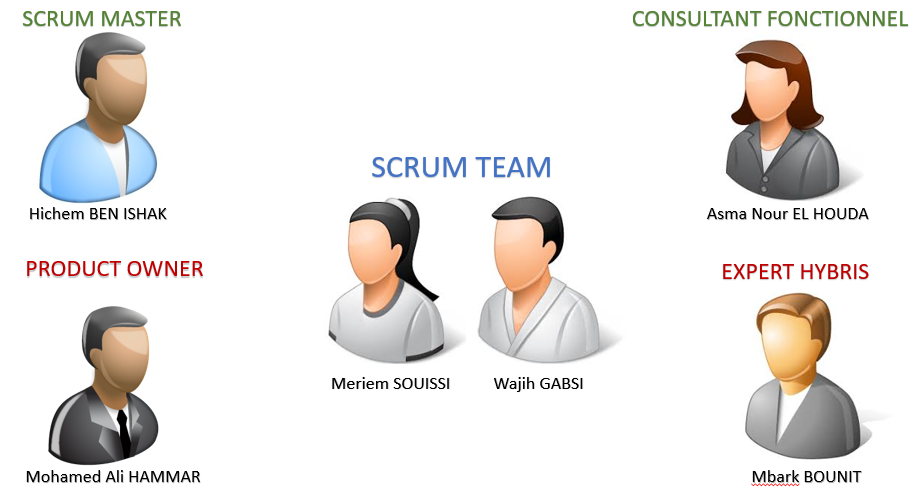
\includegraphics[width=0.7\columnwidth]{images/equipe_scrum.png}
\caption{équipe scrum}
\label{fig:Mod-Enseig}
\end{figure} 

En vue de bien mener les itérations, nous avons programmer pour chaque itération les réunions suivants :
\begin{itemize}[label=\textbullet,font=\normalsize]
\addtolength{\itemindent}{1cm}
\item \textbf{La planification du sprint }\\
Un « Sprint planning » est réalisé au début de chaque sprint, Mardi à quatorze heures. Durant cette réunion, nous décortiquons les cas d'utilisations présentés par le « product owner » en tâches techniques. Pour l’estimation des tâches, nous avons utilisé l’application mobile Scrum Poker 

\begin{figure}[H]
\centering
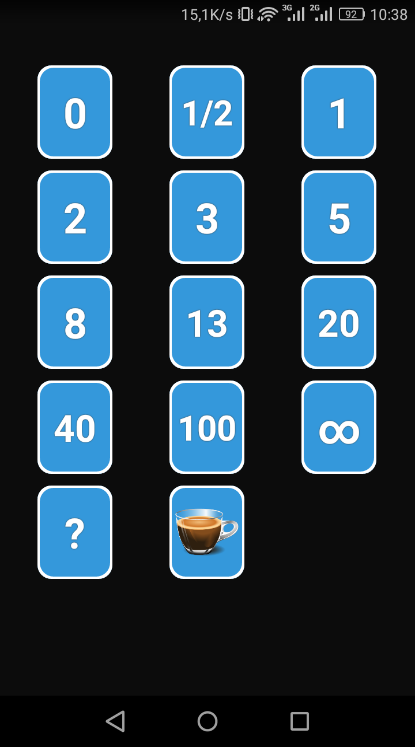
\includegraphics[width=0.29\columnwidth]{images/poker.png}
\caption{Scrum poker}
\label{fig:Mod-Enseig}
\end{figure} 

\item \textbf{La mêlée quotidienne}\\
Chaque matin nous assistons à la mêlée quotidienne pendant quinze minutes à neuf heures et quart. Durant cette réunion, le scrum master affiche le backlog produit et toute l’équipe répond chacun à ces trois questions :

\begin{itemize}[font=\normalsize]
\addtolength{\itemindent}{1cm}
\item Qu’est-ce que j’ai fait hier ? 
\item Qu’est-ce que je ferai aujourd’hui ?
\item Quels obstacles me retardent ?

\end{itemize}
\begin{figure}[H]
\centering
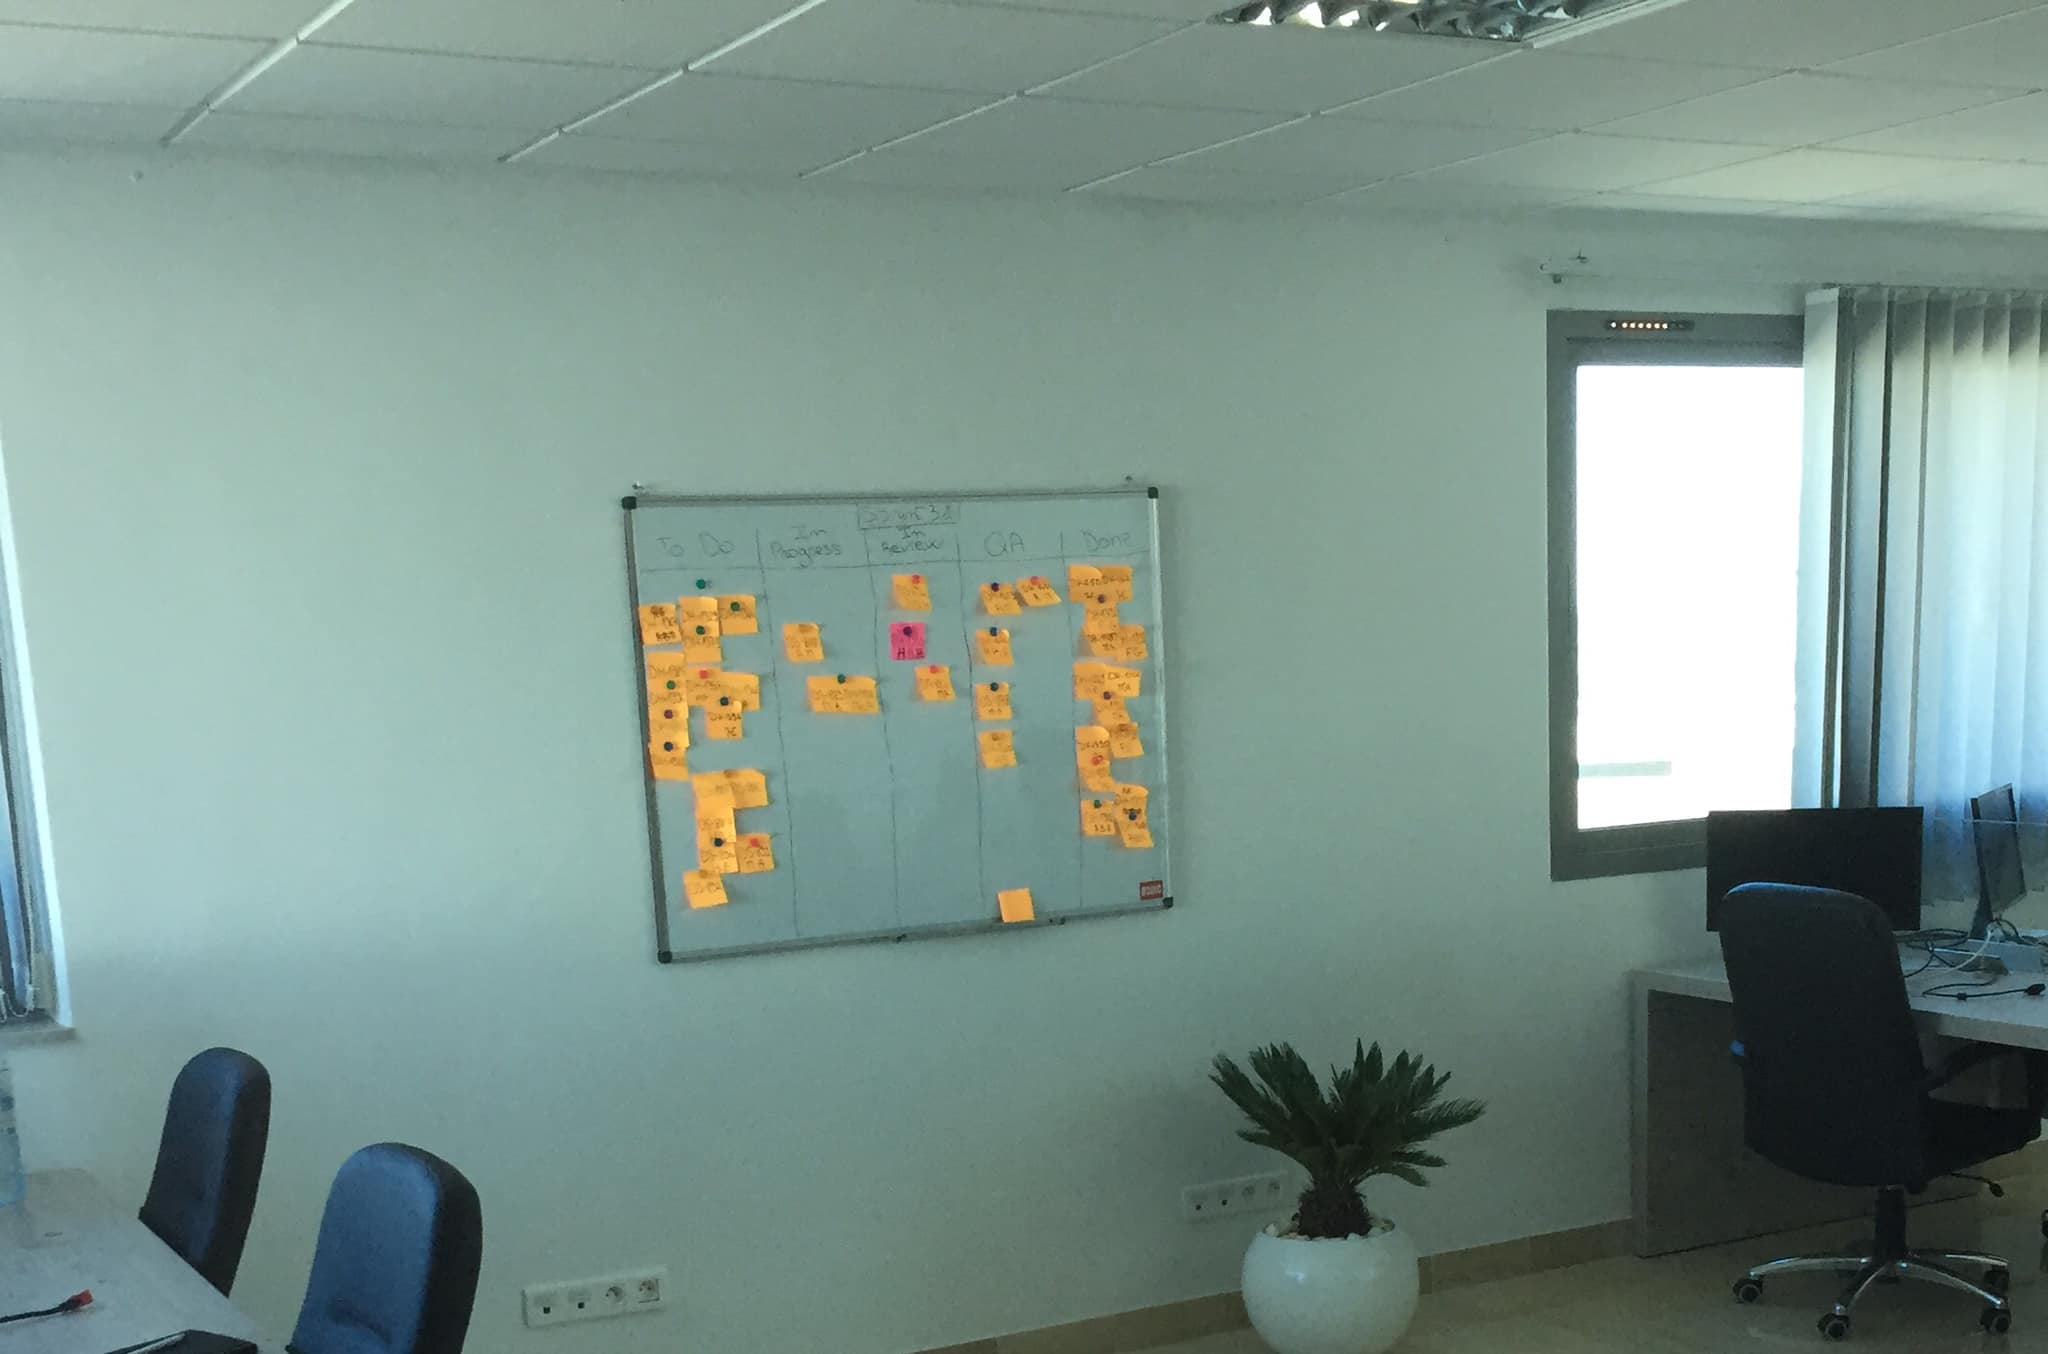
\includegraphics[width=1\columnwidth]{images/tableau1.jpg}
\caption{tableau des tâches}
\label{fig:tableau des Tâches}  
\end{figure}

\item \textbf{La revue du sprint}\\
À la fin de chaque sprint, tous les collaborateurs se réunissent pour la revue de sprint, chaque deux semaines, Le Mardi à dix heures. Durant cette réunion, nous discutons l’avancement du projet, nous évaluons les éléments finis et non finis et nous mettons à jour le Backlog produit.

\item \textbf{La rétrospective du sprint}\\
La réunion rétrospective se déroule une demi-heure juste après la revue de sprint en vue de faire le bilan de la période écoulée. Chacun évoque les points positifs et les points négatifs rencontrés tout au long du sprint.

Le schéma ci-dessous résume le processus scrum appliqué par notre équipe.

\begin{figure}[H]
\centering
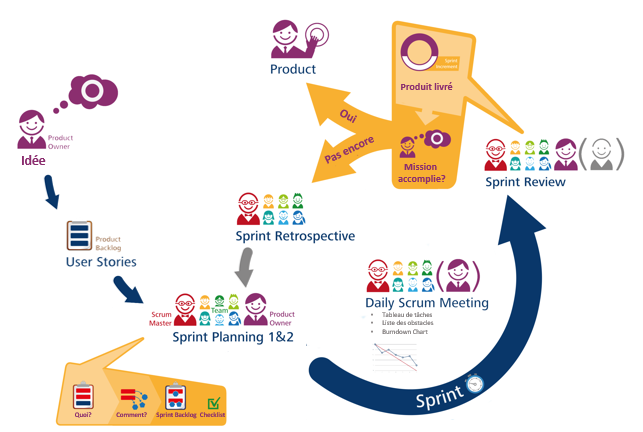
\includegraphics[width=1\columnwidth]{images/cycle_scrum.PNG}
\caption{processus scrum}
\label{fig:processus Scrum}
\end{figure} 
\end{itemize}

Notre équipe utilise l'outil Jira Agile pour la gestion du projet et des tickets, cela nous a permis de planifier et de suivre notre travail.
Les tâches sont exécutées comme suit :
Chaque tâche assignée par un membre de l’équipe doit être implémentée dans les délais définis. Ensuite nous planifions une revue de code avec un expert Hybris pour valider les spécifiés de Hybris. Si tout est validé, le code sera intégré. Finalement, la tâche sera assignée à la consultante fonctionnelle pour effectuer les tests fonctionnels nécessaires

Une tâche affectée à un développeur est une tâche en progression. Si elle est résolue, il fait un commit sur la branche d’intégration du GitLab. Dès lors, elle sera affecté au consultant fonctionnel qui doit faire les tests nécessaires, si ok elle sera validée, sinon elle sera « reopened ». Une tâche peut être en attente d'un autre évènement ou bloquée si nous n'avons pas trouvé une solution, Comme elle peut être rejetée.



\section{Les logiciels de suivi}

Pour gérer le cycle de vie du projet, nous disposons d’une chaine d’intégration continue basé sur le logiciel de suivi du projet Jira, le gestionnaire de versionning GitLab, et SonarLint l’outil de mesure de la qualité de code.

\textbf{Jira :} Le logiciel de suivi des projets, utilisé pour créer les « user stories » et les tâches. Il nous a permis aussi de planifier les sprints, d'affecter les tâches aux développeurs et d'exploiter l'avancement du développement en temps réel.

\textbf{GitLab :} Un outil dédié pour le gestionnaire de « versionning» , il permet la partage d'une base commune de travail entre les membres de l’équipe, le développement parallèle de plusieurs fonctionnalités et la gestion des conflits entre les développeurs. il permet en outre d'avoir des versions du code source sur des branches autre que la branche de déploiement.

\textbf{SonarLint :} SonarLint est un nouveau plugin officiel de SonarSource (première version datant d'octobre 2015) permettant l’analyse syntaxique du code source directement dans l'IDE en utilisant les règles d'analyse de SonarQube.
\newpage




\begin{figure}[H]
\centering
\frame{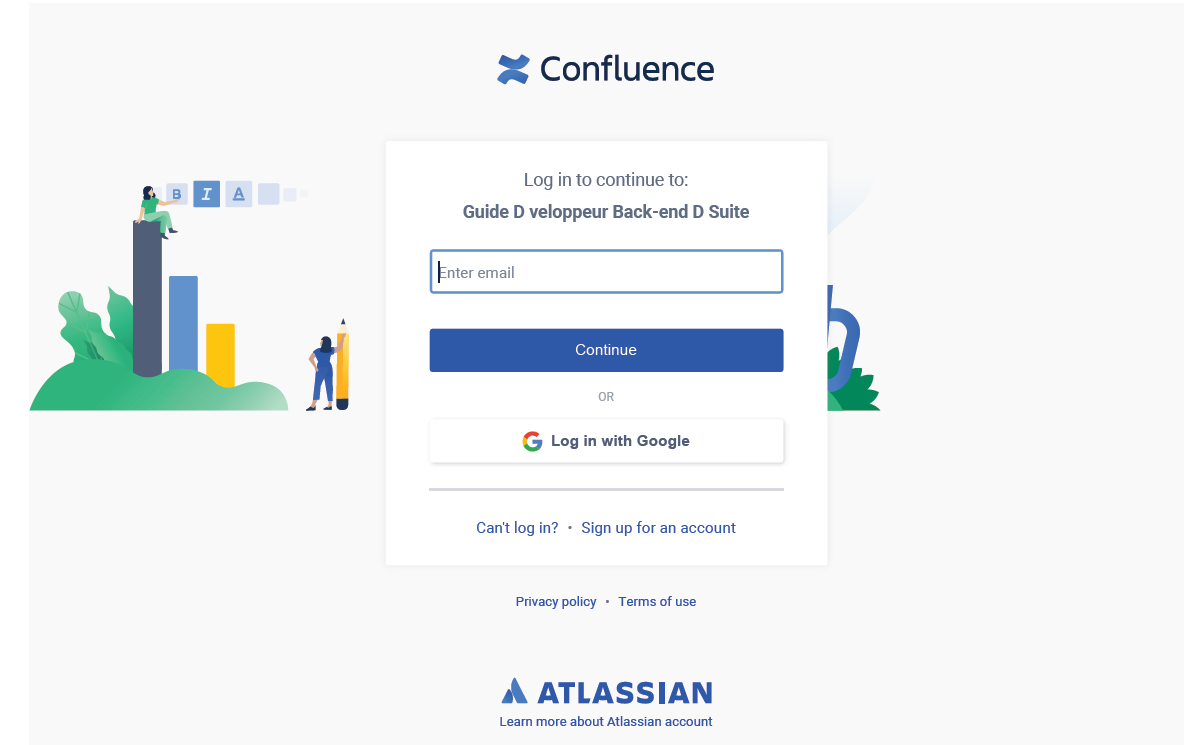
\includegraphics[width=1\columnwidth,height=0.6
\columnwidth]{images/Scrum.png}}
\caption{Jira}
\label{fig:Mod-Enseig}
\end{figure}

\section*{Conclusion}

\vspace{1cm \large Ce chapitre nous a donné l’occasion d’introduire les notions de bases de notre projet, nous avons présenté dans un premier lieu la société accueillante, puis nous avons mis le projet dans son contexte général. Puis nous avons fait une étude de l’état de l’art et enfin, nous avons établit les choix de la méthodologie appliquée dans notre projet.}
